\documentclass[aps,floatfix,10pt,amssymb,amsfont,amsmath,superscriptaddress,float,nofootinbib,longbibliography,nobalancelastpage,twocolumn]{revtex4-2}

\usepackage{color}
\usepackage{graphicx}
\usepackage{hyperref}
\usepackage{braket}
\usepackage{tikz}
\usepackage{yquant}
\usepackage[export]{adjustbox}
\begin{document}
%% Original one
% \title{Particle-to-String Conversion across Duality Defects on a Quantum Computer}
\title{Scattering Experiments on a Quantum Computer:\\
 Duality Defects and Generalized Symmetries}
\begin{abstract}
Recent advances in quantum computing provide new opportunities for studying the dynamics of excitations in quantum many-body systems. Here, we introduce a unitary protocol for preparing a localized quasiparticle wavepacket on top of the ground state. By combining this protocol with time evolution across a duality defect, we efficiently convert local particles into non-local string-like excitations, avoiding the direct implementation of extensive string operators. We demonstrate this particle-to-string conversion in the transverse-field Ising model and an SPT phase of the cluster model and implement the protocol on Quantinuum's H2 quantum computer. Our results establish duality defects and generalized symmetries as practical resources for preparing and probing non-local excitations on quantum hardware.
\end{abstract}

%%%%% Original suggestion by Oliver
% \begin{abstract}
% Duality defects separate regions that provide different local descriptions of the same underlying quantum theory. A striking prediction is that a particle incident on a topological duality defect can be transmitted while changing its operator character: an excitation that is local on one side can emerge as a non-local object attached to the defect by an extended string. This process provides a many-body realisation of the mechanism proposed to resolve the monopole-scattering paradox, in which apparently missing outgoing particles instead reside in twisted sectors of the theory.

% Here we realise this scattering process on Quantinuum's H2 trapped-ion quantum computer. We prepare momentum-resolved Gaussian wavepackets, evolve them through lattice defects implementing duality transformations, and reconstruct their propagation using local and non-local observables. For a Kramers-Wannier defect in the Ising model, a locally prepared particle crosses the interface and becomes a non-local domain-wall excitation. In a three-region construction terminating in a cluster-state symmetry-protected topological phase, the outgoing excitation disappears from local observables but remains visible through non-local string order. The continuation of the measured trajectories across the defects, together with the change in the observables required to detect them, is consistent with transmission accompanied by particle-to-string conversion. These results provide an operational quantum-computing realisation of duality-defect scattering and establish a method for studying twisted and non-local sectors of quantum many-body systems.
% \end{abstract}
\maketitle

%%%%% AU version. Maybe a bit too long? %%%%%
\section{Introduction}
Understanding quantum many-body systems is a central goal of physics, but it is rarely straightforward. Strong correlations often put these systems beyond the reach of mean-field theory or perturbative methods. Yet these systems still offer clues. One way to learn about them is to send in an excitation and see what comes back.

This is the idea behind scattering experiments. We prepare a low-energy excitation above the ground state, let it scatter, and examine the outgoing state. The result tells us both what excitations the system supports and how they interact. In many cases, an incoming particle emerges as another particle, and a single-particle scattering matrix provides a simple description.

In some systems, however, the incoming particle appears to “disappear.” The probabilities for the single-particle outcomes no longer add up to one, and the corresponding scattering matrix is non-unitary. Often, the missing probability can be accounted for by including ordinary multiparticle states. A more subtle problem arises when even this description appears insufficient. This was the difficulty encountered in the work of Callan and Rubakov on chiral fermions scattering from magnetic monopoles: the conventional fermionic description appeared to offer no outgoing state consistent with the conserved quantum numbers~\cite{Callan:1982ah,Rubakov:1982fp,Polchinski:fermion_rotor}. In this sense, an incoming fermion seemed unable to scatter back from the monopole. Of course, it is not that quantum mechanics has failed. The difficulty lies in identifying the outgoing state, a problem that became known as the “monopole paradox.”

Recent work has proposed a resolution in terms of twisted sectors~\cite{van_beest_fermion-monopole_2024,van_beest_monopoles_2025,loladze_monopole-fermion_2025,loladze_dynamics_2025}. In the effective one-dimensional description of radial scattering, the monopole acts as a boundary whose degrees of freedom participate in the scattering. The outgoing excitation belongs to a twisted sector and is attached to the monopole by a topological defect line. A unitary description therefore requires a Hilbert space that includes the monopole degrees of freedom and the relevant twisted sectors.

Although this mechanism may appear exotic, an analogous phenomenon arises naturally in quantum many-body systems in the presence of topological duality defects~\cite{ueda2025,Ueda:2026wvc}. Such a defect connects two dual descriptions of a system and can convert an incoming local excitation into its nonlocal dual. Duality matches the excitation spectra on the two sides, allowing the outgoing wavepacket to retain its energy while changing its operator representation. It can thus be understood as the same excitation in a dual description, with a topological string extending back to the interface. The degrees of freedom associated with the defect participate in this conversion and must be retained in the full scattering description.

Turning this theoretical picture into a scattering experiment on a quantum device requires control over both the incoming state and the outgoing measurement. Even when the ground state is available, preparing a localized wavepacket with a well-defined mean momentum requires a coherent superposition of excitations at different positions. After scattering, the local observables that detected the incident particle may no longer identify the outgoing excitation. Observing the conversion therefore requires efficient wavepacket preparation together with measurements tailored for the nonlocal outgoing state.

Here, we perform these scattering experiments on the Quantinuum's H2 quantum computer. We develop an efficient post-classified protocol for preparing momentum-resolved wavepackets above a many-body ground state without feed-forward or discarding valid ancilla measurement outcomes. We then implement their time evolution through duality defects and measure the outgoing dynamics using local and string observables. In two complementary lattice realizations, we reconstruct momentum-resolved space-time trajectories and follow the conversion of an incoming local excitation into an outgoing excitation with a nonlocal representation. The preparation protocol and measurements thus make these dynamics experimentally accessible on a quantum device.

The experiments also demonstrate a practical use of duality defects and generalized symmetry. Directly preparing a momentum-controlled superposition of extended string excitations can require an involved preparation circuit. By preparing a local wavepacket and allowing it to scatter from a duality defect, we instead let the dynamics generate the nonlocal excitation. The defect therefore serves as a tool for state preparation as well as an object of study, allowing access to nonlocal particle dynamics without directly preparing the corresponding string wavepacket.

The paper is organized as follows. We introduce the wavepacket-preparation protocol in Section~\ref{section:localized_wavepacket}. We then construct lattice Hamiltonians containing duality defects and study two complementary examples (Section~\ref{section:nonlocalwavepacket}). In the Ising model, a local excitation crosses a Kramers–Wannier defect and becomes a domain wall associated with a disorder string. In the cluster-model construction, the local observables that detect the incident particle no longer identify the outgoing excitation, which must instead be probed through nonlocal string-order measurements. Finally, we present the implementation on a Quantinuum's H2 quantum computer and the measured momentum-resolved space--time trajectories in Sections~\ref{section:hardwareimplementation} and \ref{section:results}.


%% Original one
% Scattering from a magnetic monopole presents a long-standing conceptual puzzle. In the Callan--Rubakov process, an incoming particle can apparently emerge with quantum numbers that do not belong to the ordinary particle spectrum of the theory. Recent work has clarified that the outgoing state is not absent, but instead belongs to a topologically twisted sector \cite{Callan:1982ah,Rubakov:1982fp}. In this sector, the excitation need not admit a local particle description and may remain connected to the monopole by a non-local string \cite{}.

% A closely related process can be realised in quantum spin systems using a duality defect. Such a defect joins regions that describe the same underlying physics in different variables. Under Kramers-Wannier duality, for example, local order operators on one side are mapped to non-local disorder strings on the other. An excitation crossing the interface can therefore be transmitted while changing its operator description: a locally created particle becomes the endpoint of an extended string in the dual region. The defect plays the role of the monopole boundary, while the outgoing string excitation realises the twisted-sector state that resolves the apparent paradox.

% This prediction has a direct operational test: prepare a wavepacket that is local on one side of a duality defect, propagate it towards the interface, and determine both whether it continues into the neighbouring region and which observables detect it after transmission. Here we perform this experiment on Quantinuum's H2 trapped-ion quantum computer. We observe momentum-resolved wavepackets crossing lattice duality defects and changing from locally prepared excitations into domain-wall or string excitations. In the cluster-model construction, the outgoing wavepacket becomes invisible to local measurements while remaining visible through non-local string order.

% Observing this conversion on a quantum computer presents a practical difficulty. The outgoing excitation is naturally represented by an extended string operator, and directly preparing a momentum-controlled superposition of such strings would require a highly non-local circuit. We avoid this cost by preparing the wavepacket in the region where the excitation is local and allowing the duality defect itself to perform the local-to-non-local conversion dynamically. The experiment therefore reproduces the scattering process rather than directly synthesising its outgoing state.

% We first introduce a post-classified protocol for preparing momentum-resolved wavepackets without feed-forward or discarding valid ancillary outcomes (Section~\ref{section:localized_wavepacket}). We then construct lattice Hamiltonians containing duality defects and show how time evolution transports a local wavepacket into sectors in which it has a non-local representation (Section~\ref{section:nonlocalwavepacket}). We study two complementary examples. In the Ising model, a local excitation crosses a Kramers-Wannier defect and becomes a domain wall associated with a disorder string. In the cluster-model construction, the outgoing excitation cannot be identified using the local observables that detected the incident particle and instead requires non-local string-order measurements. Finally, we implement both scattering experiments on the H2 quantum computer and reconstruct their momentum-resolved space--time trajectories (Sections~\ref{section:hardwareimplementation} and \ref{section:results}).

\section{Momentum-resolved wavepacket preparation}
\label{section:localized_wavepacket}
Preparing a quasiparticle wavepacket excitation on top of a many-body ground state requires implementing a non-unitary operator of the form
\begin{equation}
    \Psi_k^{\dagger} = \sum_{x=0}^{M-1} a_xe^{\frac{2\pi i}{M}kx} \phi^{\dagger}_x
\end{equation}
where $\phi^{\dagger}_x$ are unitary creation operators for localised excitations and $a_x$ are real coefficients with $\sum_{x=0}^{M-1} a_x^2 =1$.

In general, implementing a non-unitary operator such as $\Psi^{\dagger}_k$ on a quantum computer requires post-selection or mid-circuit measurement with feed-forward \cite{childs2012hamiltonian, turco2025creation, Gily_n_2019, mcardle2026quantum, o2025quantum, corcoles2021exploiting, pino2021demonstration, turco2025creation}. These approaches incur additional cost in either shot overhead or architectural complexity. We instead use a post-classification technique that retains every valid shot by preparing the state
\begin{equation}
    \frac{1}{\sqrt{M}}\sum_{k=0}^{M-1} \ket{k}\otimes\Psi_{k+k_0}^{\dagger}\ket{\Omega} 
\end{equation}
Measuring the ancilla register to be $k$ conditions the system on the application of $\Psi^{\dagger}_{k+k_0}$. We therefore prepare momentum-resolved wavepackets without discarding valid shots and without feed-forward. Although the momentum is not selected in advance, each shot can be assigned to a momentum sector from the ancilla outcome.

The circuit (shown in Fig.~\ref{fig:qcircuit}) is closely related to linear combinations of unitaries \cite{childs2012hamiltonian, berry2015simulating, babbush2018encoding} and consists of the following steps:
\begin{enumerate}
    \item \textsc{PREP}: On $m = \log_2 M$ ancillas initialised to $\ket{0}$ prepare the following state: $
            \sum_{x=0}^{M-1} a_xe^{\frac{2\pi i}{M}k_0x} \ket{x}$
    \item \textsc{SELECT}: Controlled upon this ancilla register act with $\phi^{\dagger}_x$ upon the system giving:
    $\sum_{x=0}^{M-1} a_xe^{\frac{2\pi i}{M}k_0x} \ket{x}\otimes \phi^{\dagger}_x\ket{\Omega}
    $
    \item \textsc{QFT}: Apply the quantum Fourier transform to the ancilla register, giving the final state
    \begin{multline}
       \frac{1}{\sqrt{M}} \sum_{x,k=0}^{M-1} a_xe^{\frac{2\pi i}{M}(k_0+k)x} \ket{k}\otimes \phi^{\dagger}_x\ket{\Omega} = \\\frac{1}{\sqrt{M}}\sum_{k=0}^{M-1}  \ket{k}\otimes \Psi^{\dagger}_{k+k_0}\ket{\Omega}
    \end{multline}
\end{enumerate}
\begin{figure}
    \centering
    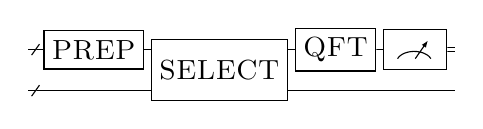
\begin{tikzpicture}
\begin{yquant*}
qubit {} anc;
qubit {} s;
slash s;
slash anc;
hspace {0.1cm} -;
box {\textsc{PREP}} anc;
box {\textsc{SELECT}} (anc, s);
box {\textsc{QFT}} anc;

measure anc;
\end{yquant*}
\end{tikzpicture}
    \caption{Quantum circuit for preparing wavepackets with post-classified momentum sectors.}
    \label{fig:qcircuit}
\end{figure}
% In Appendix~\ref{appendix} we extend this formulation to entangled multiparticle states and show in noiseless simulation that the particles retain genuine multipartite entanglement as they propagate. The entanglement is diagnosed through a Mermin inequality.
Many alternative approaches to preparing localised wavepackets exist. These include (but are not limited to): adiabatically evolving a wavepacket of a free theory into one in an interacting theory \cite{jordan2012quantum, jordan2011quantum, jordan2014quantum, brennen2014multi, barata2021single}, performing symmetry constrained variational optimization on a state with definite momentum \cite{farrell2026digital} or straight-forward variational optimization \cite{farrell2024quantum, davoudi2024scattering, zemlevskiy2025scalable}. We do not claim to outperform the state-of-the-art in wavepacket preparation, but believe our methodology may prove a valuable additional tool in particular circumstances. For example, for large systems that prove resistant to VQE techniques but for which we can efficiently prepare an approximation to the ground state our approach of applying the wavepacket on top of a prepared groundstate may be the most appropriate choice.
\section{Scattering through duality defects}
\label{section:nonlocalwavepacket}
A duality defect changes the operator description of an excitation without changing the underlying propagating degree of freedom. Consequently, a wavepacket created by local operators on one side of the interface may be represented by a string operator on the other. 

Our experiment exploits this property directly. We prepare the incident wavepacket in a region where it is local, evolve it towards the defect, and reconstruct the outgoing excitation using observables appropriate to the dual region. This avoids direct preparation of a superposition of extensive strings.

Generalised symmetries provide the formal structure for this construction. A model with non-local excitations can admit a dual description in which the same excitations are localised \cite{}. In one dimension, the intertwiner between such dual models can be represented as a matrix-product operator (MPO) \cite{lootens2023dualities, lootens2024dualities}. Joining the two descriptions with the corresponding defect yields an interface across which the ideal wavepacket is perfectly transmitted \cite{ueda2026perfect, ueda2026emergent}. The defect can therefore be viewed as a boundary between different topological sectors, analogous to the role played by the monopole in the motivating scattering problem.

\subsection{Example models}
We realise the scattering process in two complementary models. The Ising construction converts a local particle into a domain-wall wavepacket whose preparation is non-local but which remains detectable through a local order parameter. The cluster model construction converts a locally visible particle into a string excitation in a symmetry-protected topological (SPT) phase, where it is detected through non-local string order.

\subsubsection{Ising Model: conversion into a domain wall}
\begin{align*}
H_{i} &= H_1 \;+\; H_2 \;+\; H_{\mathrm{im}}^{(L)} \;+\; H_{\mathrm{im}}^{(R)}, \\[6pt]
H_1
&= -\sum_{j=0}^{I_L-1} Z_j
\;-\; g \sum_{j=0}^{I_L-2} X_j X_{j+1} \\[4pt]
&\quad -\; \sum_{j=I_R+1}^{L-1} Z_j
\;-\; g \sum_{j=I_R+1}^{L-2} X_j X_{j+1}\\
%
H_2
&= -\sum_{j=I_L+1}^{I_R-2} Z_j Z_{j+1}
\;-\; g \sum_{j=I_L+1}^{I_R-1} X_j, \\[8pt]
%
H_{\mathrm{im}}^{(L)}
&= - Z_{I_L} Z_{I_L+1}-g X_{I_L-1} X_{I_L}, \\[6pt]
%
H_{\mathrm{im}}^{(R)}
&= - Z_{I_R-1} Z_{I_R}
\;-\; g\, X_{I_R} X_{I_R+1}.
\end{align*}

% At first this Hamiltonian may seem contrived, however, after applying a modified Jordan-Wigner transformation it has a much clearer representation in terms of Majorana fermions.
% \begin{multline}
%     H = \sum_{j=0}^{2I_L-2} \gamma_{j}\gamma_{j+1} + \gamma_{2I_L-1}\gamma_{2I_L+1} + \\\sum_{j=2I_L+1}^{2I_R-1} \gamma_j\gamma_{j+1} + \gamma_{2I_R}\gamma_{2I_R+2} + \\\sum_{j=2I_R+2}^{2L-2}\gamma_j\gamma_{j+1} + \gamma_{2L-1}\gamma_0
% \end{multline}
% Under this representation it is clear that the impurities arise due to uncoupled majorana modes $\gamma_{2I_L}$ and $\gamma_{2I_R+1}$. Therefore, by relabeling the majoranas we could rewrite $H$ as:
% \begin{equation}
%     H = \sum_{j=0}^{2L-3} \gamma_j\gamma_{j+1} + \gamma_{2L-3}\gamma_0
% \end{equation}
% This is equivalent to 

$H_1$ and $H_2$ provide order and disorder descriptions of the same Ising quasiparticle, with the MPO intertwiner between them given by Kramers-Wannier duality. The overall Hamiltonian $H_i$ is obtained by applying this duality to a transverse-field Ising model with two maximally entangled defect sites, as illustrated below:

\begin{equation}
    \centering
\begin{array}{c}

H_i =\>\>\includegraphics[width=0.5\linewidth, page=2, valign=c]{figs/figs.pdf} \\
\\
\big\downarrow \\
\\
H_i =\>\> \includegraphics[width=0.3\linewidth, page=3, valign=c]{figs/figs.pdf}

\end{array}
\end{equation}

The two regions describe the same underlying excitation in different sectors. In $H_1$, the incident wavepacket is created by a superposition of local Pauli-$X$ operators. After crossing a Kramers-Wannier defect into $H_2$, the corresponding excitation is a propagating domain wall and is therefore non-local. The defect thus converts a local particle into a non-local particle while preserving its propagation through the system.

Because the Kramers-Wannier duality preserves the spectrum and dynamics of the original model, the ideal construction predicts perfect transmission across both defect sites. The outgoing state is not a different wavepacket created at the boundary, but the dual representation of the incident excitation. The wavepacket subsequently encounters a second Kramers-Wannier defect; crossing this interface reverses the transformation and returns the excitation to a local representation. The full trajectory therefore realises a particle-to-string-to-particle scattering sequence.

% In order to probe the non-trivial physics of these non-local wavepackets we will instigate a quench some time after the wavepacket has crossed into $H_2$ by introducing an additional local longitudinal field. The quenched Hamiltonian $H_2'$ is given by:
% \begin{align*}
%    H_2' = &-\sum_{j=0}^{I_L-1} X_j
% - g \sum_{j=0}^{I_L-2} Z_j Z_{j+1} \\
% & - \sum_{j=I_R+1}^{L-1} X_j
% - g \sum_{j=I_R+1}^{L-2} Z_j Z_{j+1}\\
% &- g Z_{L-1} Z_0 \\
% &- g_z \sum_{j=0}^{I_L-1} Z_j - g_z \sum_{j=I_R+1}^{L-1} Z_j
% \end{align*}
% This longitudinal field makes the model non-integrable and acts as an effective ``tension" in the string-like excitation. Implementing this quench breaks the duality between $H_1$ and $H_2$ leading to a confinement of the non-local excitation to the dual theory. Therefore, due to the ``tension" in the string we observe a wavepacket oscillating back-and-forth from the boundary of $H_2$.
\subsubsection{Cluster model: conversion into an SPT string excitation}
In the Ising construction, the outgoing domain wall requires a non-local superposition of operators for direct preparation but remains detectable through a local order parameter. We now introduce a three-region model that separates propagation from local visibility more sharply: after crossing the second defect, the excitation propagates on top of the cluster state and is detected through non-local string-order parameters rather than the original local observables:

\begin{align*}
    H_{c} &= H_1 + H_2 + H_3 + H_{im}^{(L)} + H_{im}^{(R)}\\
    H_1 &=-\sum_{j=0}^{I_L-1} Z_j- g\sum_{j=0}^{I_L-3}X_jX_{j+2}  \\
    H_2 &=- \sum_{j=I_{L}+2}^{I_R-3} Z_{j}Z_{j+2} -g \sum_{j=I_{L}+2}^{I_R-1} X_j\\
    H_3 &= - \sum_{j=I_R+1}^{L-3}Z_j X_{j+1}Z_{j+2} - g \sum_{j=I_R+1}^{L-1}  X_j\\
    H^{(L)}_{im} &= -Z_{I_L}Z_{I_L+2} - Z_{I_L+1}Z_{I_L+3}\\
    &\;\;-g X_{I_L-2}X_{I_L} -g X_{I_L-1} X_{I_L+1}\\
    H^{(R)}_{im} &= -Z_{I_R-2}Z_{I_R}Z_{I_R+1} - Z_{I_R-1}X_{I_R}X_{I_R+1}Z_{I_R+2}
\end{align*}

This model consists of a pair of interleaved open-boundary transverse-field Ising chains transformed by three dualities. First, two copies of Kramers-Wannier duality are applied to the left-hand side of the chains, relating their paramagnetic and ferromagnetic descriptions as in the preceding construction. Second, a spin-$\frac{1}{2}$ analogue of the Kennedy-Tasaki transformation \cite{li2023noninvertible} is applied to the right-hand side of both chains, producing a single $ZXZ$ cluster model. The Kennedy-Tasaki transformation is represented by an MPO constructed from two tensors:
\begin{equation}
    \includegraphics[page=4, valign=c]{figs/figs.pdf} = \sum_{a,j=0}^1(-1)^{aj} \ket{a}\bra{a} \otimes \ket{j}\bra{j}
\end{equation}
\begin{equation}
    \includegraphics[page=5, valign=c]{figs/figs.pdf} = \sum_{a,j=0}^1 \ket{a\oplus j}\bra{a} \otimes \ket{j}\bra{j}
\end{equation}
These combine together into the following Kennedy-Tasaki MPO:
\begin{equation}
    \includegraphics[page=6]{figs.pdf}
\end{equation}
Applying this transformation to the pair of interleaved open-boundary Ising chains, after Kramers-Wannier duality has been applied on their left-hand side, produces $H_c$:
\begin{equation}
    H_{c}=\includegraphics[width=0.8\linewidth, page=8, valign=c]{figs/figs.pdf}
\end{equation}

The $H_3$ cluster model realises a one-dimensional $\mathbb{Z}_2\times \mathbb{Z}_2$ SPT phase whose ground state at $g=0$ is the cluster state. This SPT phase extends to $g<1$, where the ground state is no longer the simple fixed-point cluster state. A wavepacket created locally in $H_1$ first becomes a domain wall in $H_2$ and then a non-local string excitation propagating through the SPT phase in $H_3$. Unlike the Ising construction, the two defects implement different transformations, so the outgoing excitation does not return to its original local description.

This construction provides a direct experimental test of whether a particle that disappears from local observables has been destroyed or has instead entered a non-local sector. Before reaching the second defect, the wavepacket can be tracked using the original local observables. After entering $H_3$, the same propagating excitation cannot be detected by the original local observables but is detected using the non-local string order inherited from the duality transformation.

\subsection{Experimental implementation}
\label{section:hardwareimplementation}
To implement the scattering dynamics of both models on quantum hardware, we
\begin{enumerate}
    \item prepare an approximation to the many-body ground state,
    \item excite a local wavepacket on top of this background,
    \item evolve the wavepacket through the duality defects, and
    \item measure the outgoing excitation using the appropriate local or non-local observable.
\end{enumerate}
Each step is adapted to reduce the circuit depth and measurement cost on current quantum hardware.

\subsubsection{Ground state preparation}
Matrix-product-state (MPS) representations of the ground states can be found efficiently and to high precision using DMRG \cite{PhysRevLett.69.2863,schollwock2011density}. We then use AQCtensor \cite{robertson2025approximate} to obtain low-depth circuits that approximate these states. The method begins with a parameterised hardware-efficient ansatz, compresses it into an MPS using tensor-network simulation, and evaluates its fidelity with the target ground-state MPS. Standard numerical optimisation, such as L-BFGS-B, then converges to a low-depth approximation. We use a low-depth ansatz circuit tailored to the connectivity of the model of interest. For the Ising model, we use pairwise rZZ interactions interspersed with rX rotations. For the Cluster model, we use a tailored ansatz of two separate chains of next-nearest neighbour rZZ interactions until $I_R$ when we transition into a single chain of pairwise rZZ interactions, again interspersed with rX rotations. Figure~\ref{fig:groundstateprep} shows the dependence of the ground-state preparation error on circuit depth. Based on this data, we use an ansatz with a two-qubit depth of 8 for the Ising model and 9 for the cluster model. 
\begin{figure}
    \centering
    \includegraphics[width=0.8\linewidth]{figs/gs_fid.png}
    \caption{Ground-state preparation error for the Ising model and Cluster model on a 36-qubit system at $g=0.7$ as a function of the two-qubit depth of the optimised hardware-efficient ansatz $V(\theta)$. The vertical axis shows the infidelity between the variationally prepared state $V(\theta)\ket{0}$ and the target DMRG/MPS ground state $\ket{\psi}$. We also show the estimated error due to hardware noise introduced by including one additional layer in the ansatz.}
    \label{fig:groundstateprep}
\end{figure}
\subsubsection{Wavepacket preparation}
We implement the protocol of Section~\ref{section:localized_wavepacket} with several modifications for current quantum hardware.

First, the standard implementation of \textsc{SELECT} requires expensive multiplexed controlled unitaries. We instead use a unary encoding of the ancilla register. At the cost of additional ancillas, this reduces \textsc{SELECT} to $M$ two-qubit \textsc{CNOT} gates. In the $H_1$ region, where the incident wavepacket is created, the localised excitation $\phi_i^\dagger$ is a Pauli $X$ operator on site $i$ for both models.

Second, for Gaussian wavepackets, \textsc{PREP} prepares the state
\begin{equation}
    \frac{1}{\mathcal{N}}\sum_{x=0}^{M-1}e^{-\left(\frac{x-\frac{M-1}{2}}{\sigma}\right)^2}e^{\frac{2\pi i}{M}k_0 x} \ket{2^x}
\end{equation}
Because the Gaussian tails decay exponentially, we can take $M\ll L$ with little truncation error. We approximate \textsc{PREP} by numerically optimising a hardware-efficient variational ansatz at modest classical cost.

The unary encoding also changes the implementation of \textsc{QFT}. We use the shallow-depth unary QFT circuit proposed in Ref.~\cite{jain2024quantum}, which replaces the radix-2 operations in the Cooley-Tukey fast Fourier transform \cite{cooleytukey} with two-qubit gates. It requires $n\log n$ two-qubit gates and benefits from the all-to-all connectivity of the trapped-ion architecture. 

Finally, the unary encoding provides a simple error-detection condition: we discard ancillary outcomes whose Hamming weight is not one.

\subsubsection{Time evolution}
We implement time evolution using a second-order Suzuki-Trotter decomposition \cite{suzuki1976generalized, suzuki1991general} whereby time evolution by a target Hamiltonian $H=\sum_j h_j$ is performed through the symmetrised operator:
\begin{equation}
   e^{-iHt} \approx \left(e^{\frac{ -ih_1 t}{2r}}\cdots e^{\frac{ -ih_{L-1} t}{2r}}e^{\frac{ -ih_L t}{r}} e^{\frac{ -ih_{L-1} t}{2r}}\cdots e^{\frac{ -ih_1 t}{2r}}\right)^r
\end{equation}
The operator error of this approximation can be bounded as $\epsilon_T=O\left(\frac{t^3}{r^2}\sum_{j,k,l}\|[h_l,[h_j,h_k]]\|\right)$ \cite{childs2021theory}. For local models we have $\sum_{j,k,l}\|[h_l,[h_j,h_k]]\|=O(L)$ and hence evolving to time $t$ with $r$ timesteps we get $\epsilon_T=O\left(\frac{L t^3}{r^2}\right)$.

For our circuits we can choose an ordering such that our second-order trotter circuit has almost the same depth as a first-order trotter circuit \cite{layden2022first}. This is seen by grouping our Hamiltonian into two parts ($H_\alpha$, $H_\beta$) such that every term in each part commutes with every other term in the part. Then we can see that the second-order trotter circuit can be written as:
\begin{equation}
    \left(e^{\frac{ -iH_\alpha t}{2r}}e^{\frac{ -iH_\beta t}{r}} e^{\frac{ -iH_\alpha t}{2r}}\right)^r = e^{\frac{ -iH_\alpha t}{2r}}\left(e^{\frac{ -iH_\beta t}{r}} e^{\frac{ -iH_\alpha t}{r}}\right)^r e^{\frac{ iH_\alpha t}{2r}}
\end{equation}
Therefore, we can achieve second-order trotter error scaling with ``almost" first-order trotter circuits. We further reduce the depth of our circuits by ensuring every trotter step is optimally parallelised.
\subsubsection{Measurement}
In the Ising model, the outgoing domain wall can be detected through a local order parameter, so we measure all system qubits in the $Z$ basis. In the cluster model, detecting the transmitted excitation is instead detected through the non-local order parameters $S_i$
\begin{equation}
S_i = \begin{cases}Z_{I_R}Z_{i}\prod_{j=1}^{\frac{i-I_R-1}{2}}X_{I_R+2j} & \text{for odd } (i-I_R)\\
    X_{I_R}Z_{i}\prod_{j=1}^{\frac{i-I_R-2}{2}}X_{I_R+2j+1} &\text{for even }  (i-I_R)
    \end{cases}
    \label{eq:Si}
\end{equation}
Strings terminating on sites of the same parity commute qubit-wise. Therefore, splitting them into even and odd groups allows all string-order expectation values to be evaluated using two measurement settings:
\begin{equation}
    Z_{I_R}\prod_{j=I_R+1}^{L-2} Z_{j}X_{j+1} \;\text{ and }\;  X_{I_R}\prod_{j=I_R+1}^{L-2} X_{j}Z_{j+1}
\end{equation}
The non-local wavepacket can therefore be reconstructed with two measurement circuits per evolution time.
\begin{figure*}
    \centering
    \includegraphics[width=\linewidth]{figs/isingmodel.png}
    \caption{Momentum-resolved transmission and particle-to-domain-wall conversion across Kramers-Wannier duality defects on the Quantinuum H2 quantum computer, with $g=0.7$, $I_L=16$, $I_R=19$, and $L=36$. Each panel shows the mean $Z$-basis measurement outcome as a function of lattice site and evolution time, conditioned on the measured unary-ancilla momentum outcome $k$ (where $\tilde k =\frac{2\pi}{M}(k+k_0)$ with $M=8$). The 300 shots performed are split between the 8 post-classified panels. The wavepacket begins as a superposition of local Pauli-$X$ excitations in $H_1$. After crossing a defect into $H_2$, it is represented as the endpoint of a non-local disorder string and is interpreted as a propagating domain wall. When it crosses back to $H_1$ it again becomes localised. The predicted ballistic trajectory is given by the group velocity of the central momentum $\tilde k$ of each wavepacket. As the wavepackets are localised in space they are spread in momentum space and hence actually contain a range of group velocities. We are using linear interpolation to smooth out the hardware plots as we only measured the six distinct timesteps detailed in Table~\ref{tab:trotter_steps}.}
    \label{fig:isingmodel}
\end{figure*}
\begin{figure*}
    \centering
    \includegraphics[width=\linewidth]{figs/mpsising.png}
    \caption{MPS simulation of wavepacket propagation on the Ising model with a Kramers-Wannier duality defect for a range of $g$ values for the dual model ($H_2$). Each panel shows the interpolated mean $Z$-basis outcome as a function of lattice site and evolution time. Every panel uses the same central momentum of $\tilde k = 0.44\pi$ to minimise the spread of group velocities. Perfect transmission is observed for $g=0.7\rightarrow 0.7$ (a) in accordance with Fig.~\ref{fig:isingmodel}f. Partial transmission is observed for $g=0.7\rightarrow 0.4$ (b) and complete reflection is observed for $g=0.7\rightarrow0.1$ (c).}
    \label{fig:mpsising}
\end{figure*}

\begin{figure*}
    \centering
    \includegraphics[width=\linewidth]{figs/cluster_model.png}
    \caption{Conversion of a locally visible particle into a non-local string excitation across sequential duality defects of $H_c$ on the Quantinuum H2 quantum computer, with $g=0.7$, $I_L=15$, $I_R=23$, and $L=36$. The columns show four post-classified momentum sectors conditioned on the measured unary-ancilla momentum outcome $k$ (where $\tilde k =\frac{4\pi}{M}(k+k_0)$ with $M=8$). The upper row displays the mean $Z$-basis measurement outcome, while the lower row displays the mean non-local string-order signal $\braket{S_i}$ defined in Eq.~\ref{eq:Si} (with $S_i = Z_i$ to the left of $I_R$). Before the wavepacket enters the cluster region, its trajectory is visible locally. After crossing the second defect at $I_R$, the propagating feature disappears from the local signal but continues in the string-order measurements. The complementary signals show that the excitation has entered the SPT region while changing from a locally detectable particle into a non-local string excitation. We are using linear interpolation to smooth out the hardware plots as we only measured the six distinct timesteps detailed in Table~\ref{tab:trotter_steps}. Two measurement settings were used to produce these plots with 400 hardware shots post-classified over the four panels in each row. For sites to the left of $I_R$ the two measurement settings coincide so there are effectively 800 hardware shots split over each row.}
    \label{fig:clustermodel}
\end{figure*}
\begin{figure*}
    \centering
    \includegraphics[width=\linewidth]{figs/ising_model_slices.png}
    \includegraphics[width=\linewidth]{figs/cluster_model_slices.png}
    \caption{Time slices from Fig~\ref{fig:isingmodel}(f) and Fig.~\ref{fig:clustermodel}(g) showing the comparison between the hardware shots (with Clopper–Pearson 95\% confidence intervals) and an MPS simulation for $\tilde k = 0.44\pi$. We see strong agreement between the results from the quantum device and the classical simulation.}
    \label{fig:slices}
\end{figure*}
\subsection{Results}
\label{section:results}
We now test the defining prediction of duality-defect scattering: whether a wavepacket continues through the interface while changing from a local excitation into a domain-wall or string excitation. 

We perform both experiments on Quantinuum's 56-qubit H2 trapped-ion quantum computer. The Ising and cluster-model are both considered for $g=0.7$ and we compute the time evolution to a range of times using different numbers of trotter steps given by Table~\ref{tab:trotter_steps}.
\begin{table}[htbp]
    \centering
    \begin{tabular}{|c|c|c|c|}
    \hline
        \multicolumn{4}{|c|}{\textsc{Ising Model}} \\\hline
         \textbf{Time}& \textbf{Trotter steps}&\textbf{2 qubit gate count}&\textbf{Post-selection}  \\\hline
         0.00&0&193&96.7\%\\\hline
         1.70&3&355&75.7\%\\\hline
         3.40&6&460&78.3\%\\\hline
         5.10&9&577&88.7\%\\\hline
         6.80&12&688&86.7\%\\\hline
         8.50&15&799&91.3\%\\\hline
    \end{tabular}\vspace{1cm}
    \begin{tabular}{|c|c|c|c|}
    \hline
     \multicolumn{4}{|c|}{\textsc{Cluster Model}} \\\hline
         \textbf{Time}& \textbf{Trotter steps}&\textbf{2 qubit gate count}&\textbf{Post-selection}  \\\hline
         0.00&0&156&97.4\%\\\hline
         1.67&4&368&92.6\%\\\hline
         3.33& 7&476&90.1\%\\\hline
         5.00&10&585&91.9\%\\\hline
         6.67&14&729&91.4\%\\\hline
         8.33&17&837&90.2\%\\\hline
         % 10.00&20&945&\\\hline
    \end{tabular}
    \caption{Tables illustrating the various time steps evaluated in the quantum time evolution of each model along with the number of trotter steps and 2 qubit gates used in such evaluation. The post-selection proportion corresponds to the proportion of samples that are measured with hamming weight 1 and hence are retained into the plots. This is an effective error mitigation strategy for detecting bit flip errors in the ancillas.}
    \label{tab:trotter_steps}
\end{table}

For the Ising model, we choose the optimal $k_0$ to minimise the spread of the group velocities within the wavepacket. In the idealised case this would be given by $\arccos g$, however due to the non-zero width of our wavepacket this is no longer optimum. Using the dispersion relation for the Ising model we numerically calculated the optimum $k_0$ for our wavepacket width to be given by $\tilde k_0 = \frac{2\pi }{M}k_0=0.44\pi$.

The localised wavepacket created in the cluster model is
\begin{equation}
    \Psi_k^{\dagger} = \sum_{p=0}^{M-1} e^{-\left(\frac{p-\frac{M-1}{2}}{\sigma}\right)^2}e^{\frac{2\pi i}{M}k p} X_p 
\end{equation}
Because the model consists of two Ising chains on the odd and even sites, this can be written as
\begin{equation}
    \Psi_k^{\dagger} = \Psi_{k,1}^{\dagger} +\Psi_{k,2}^{\dagger}
\end{equation}
where
\begin{equation}
        \Psi_{k,1}^{\dagger} = \sum_{p=0}^{\frac{M-2}{2}} e^{-\left(\frac{2p-\frac{M-1}{2}}{\sigma}\right)^2}e^{\frac{4\pi i}{M}k p} X_{p,1} 
\end{equation}
\begin{equation}
        \Psi_{k,2}^{\dagger} = \sum_{p=0}^{\frac{M-2}{2}} e^{-\left(\frac{2p+1-\frac{M-1}{2}}{\sigma}\right)^2}e^{\frac{2\pi i}{M}k (2p+1)} X_{p,2} 
\end{equation}
The central momentum of these wavepackets is therefore $\tilde k =\frac{4\pi}{M}k$ rather than $\frac{2\pi}{M}k$. Pairs of ancilla outcomes correspond to the same effective momentum, and we choose $\frac{2\pi }{M}k_0=0.22\pi$ to minimise the spread of group velocities.

Both experiments use a wavepacket width of 8. We allocate $M=8$ ancillas to the unary register and $L=36$ qubits to the spin lattice. Post-classifying the circuit outcomes by the measured ancilla bits gives eight momentum sectors for the Ising model and four for the cluster model, where the reduction follows from the degeneracy associated with the two interleaved Ising chains.

Figures~\ref{fig:isingmodel} and \ref{fig:clustermodel} show the resulting space-time trajectories. Reversing the sign of the post-classified momentum reverses the direction of propagation, while changing its magnitude changes the trajectory slope, as expected from the momentum-dependent quasiparticle group velocity. A Gaussian wavepacket in position space also has a finite momentum width and consequently the momentum sectors with small group velocity contain components with both signs of velocity and display broader bidirectional signals.

Figure~\ref{fig:isingmodel} shows the scattering of the Ising wavepacket through the Kramers-Wannier defects. The wavepacket is initially prepared as a superposition of local Pauli-$X$ excitations in $H_1$. Its diagonal space-time trajectory continues across the interface into $H_2$, where Kramers-Wannier duality maps the excitation to a non-local domain wall. No separate reflected branch is resolved at the interface, and the continuation of the trajectory is consistent with the transmission expected for the ideal duality defect. Because the domain wall remains detectable through the local Ising order parameter, it can still be followed after entering the dual region. Crossing the second defect returns the wavepacket to a local representation. We contrast Fig.~\ref{fig:isingmodel} with Fig.~\ref{fig:mpsising} which demonstrates that when the model and dual model do not match across the defect we do not observe perfect transmission, and for a large enough difference in parameters we observe perfect reflection.

Figure~\ref{fig:clustermodel} provides the clearest distinction between propagation and local observability. Before the wavepacket crosses the second defect, its trajectory is visible in the local $Z$-basis signal. After it enters the cluster region, the propagating feature disappears from this local observable. Taken alone, the loss of local contrast could be interpreted as absorption, decoherence, or reflection at the interface. The non-local string-order measurements show instead that the trajectory continues into the SPT region with the same direction of propagation. The particle has therefore not simply disappeared; the defect has transformed it into an excitation whose presence is encoded non-locally along a string extending from the interface. This is the lattice mechanism corresponding to the transfer of an outgoing particle into the twisted sector invoked in resolutions of the monopole paradox.

A useful feature of post-classification is that one family of circuits provides access to every momentum sector shown in Figs.~\ref{fig:isingmodel} and \ref{fig:clustermodel}. Each outcome satisfying the unary Hamming-weight constraint is retained and assigned to its corresponding value of $k$. 

Figure~\ref{fig:slices} highlights particular time slices from Fig.~\ref{fig:isingmodel} and Fig.~\ref{fig:clustermodel} for the optimum central momentum to minimise the spread of group velocities. We can see how the hardware results closely agree with the classical MPS simulation for both models.


\section{Discussion}

We have implemented the scattering of momentum-resolved wavepackets through duality defects on a programmable trapped-ion quantum computer. These defects are not conventional impurity potentials, but interfaces between different operator descriptions of the same underlying quantum theory. Their defining effect is therefore not merely a change in the velocity or amplitude of a wavepacket, but a change in the type of operator required to describe the outgoing excitation.

In the Ising experiment, a wavepacket prepared from local spin excitations propagates through a Kramer-Wannier defect and enters the dual region as a domain wall associated with the endpoint of a disorder string. The continued space-time trajectory and the absence of a separately resolved reflected branch are consistent with the perfect-transmission property of the ideal defect. Because the domain wall remains detectable through a local order parameter, this construction permits the particle-to-string-to-particle sequence across the two defects to be followed directly.

The Cluster model experiment provides a sharper distinction between propagation and local observability. Once the excitation enters the SPT region, it disappears from the local $Z$ signal but remains visible through non-local string order. The complementary behaviour of these measurements shows that the wavepacket has not simply been lost at the interface. Instead, its information has been transferred into a non-local excitation extending across multiple sites. In the language of duality defects, the same physical excitation has entered a sector in which it no longer admits the original local particle description.

This process realises, in a controllable quantum many-body system, the mechanism proposed to resolve the monopole-scattering paradox. In monopole scattering, the apparent absence of an allowed outgoing particle can be understood by recognising that the final state belongs to a twisted sector and remains non-locally connected to the monopole. Here the duality defect plays the role of the sector boundary: an incoming local excitation crosses the interface and emerges as the endpoint of a string. 

% The experiment should therefore be understood not as a simulation of a microscopic magnetic monopole, but as a quantum-computing realisation of the topological scattering mechanism responsible for the change in particle identity.

The experiment also gives an operational role to dualities and generalised symmetries. Rather than using a duality only as a formal relation between Hamiltonians, we use its defect as a dynamical device that converts experimentally accessible local states into otherwise costly non-local states. The wavepacket is prepared where it is local, and the defect generates its non-local representation through time evolution. This viewpoint may extend to other MPO dualities and to systems containing symmetry defects, disorder operators, anyonic strings, or topological boundary conditions.

% The present data establish a proof of principle rather than a precision measurement of scattering amplitudes. The ideal construction predicts unit transmission, whereas the hardware data show a continuous transmitted trajectory with no separately resolved reflected component. A quantitative test would require extracting transmission and reflection coefficients, with uncertainties, and comparing them with exact and noiseless Trotter simulations. Higher-order product formulas, larger lattices, and longer propagation times would help separate transmitted and reflected components and reduce finite-size recurrences.

% Several further extensions are natural. Mid-circuit measurement and feed-forward could directly select a desired momentum sector when obtaining all sectors simultaneously is unnecessary. A longitudinal-field quench in the Ising construction could give the disorder string an effective tension and enable a direct study of confinement. The multiparticle extension in Appendix~\ref{appendix} also suggests a route to preparing spatially separated, momentum-entangled particles and tracking the transport of multipartite entanglement through duality defects.

Taken together, the results show a particle crossing a duality interface and changing from a local excitation into a domain-wall or string excitation. They provide a quantum-computing implementation of the particle-to-twisted-sector conversion underlying the modern resolution of the monopole paradox and demonstrate that an apparently missing particle can remain present in observables that are intrinsically non-local.
\bibliography{ref}
% \appendix
% \section{Entangled Wavepacket Preparation}
% \label{appendix}
% Our methodology for preparing localised wavepackets can be extended to entangled multi-particle states. For example, for an entangled two particle system we can prepare the following state:
% \begin{equation}
%     \frac{1}{M}\sum_{k,k'=0}^{M-1}\ket{k}\otimes \Psi_{k_0+k'}^{A\dagger}\Psi_{k-k'}^{B\dagger} \ket{\Omega}
% \end{equation}
% Here when measuring the ancilla register to be $k$, we find we have applied $\sum_{k'} \Psi_{k_0+k'} \Psi_{k-k'}$. Thus we have created a pair of particles entangled through their momentum such that their total momentum is given by $k_0+k$.

% This is achieved through a simple modification of the existing protocol in the \textsc{SELECT} step. Here instead of acting with $\phi_x^{\dagger}$ we act with $\phi^{A\dagger}_x\phi^{B\dagger}_x$ thereby creating the state: $\sum_{x=0}^{M-1} a_xe^{\frac{2\pi i}{M}k_0x} \ket{x}\otimes \phi^{A\dagger}_x\phi^{B\dagger}_x\ket{\Omega}$. Therefore, after acting with \textsc{QFT} we are left with:
% \begin{equation}
%     \frac{1}{\sqrt{M}}\sum^M_{x,k=0} a_x e^{ \frac{2\pi i}{M}(k_0+k) x}\ket{k}\otimes \phi^{A\dagger}_x\phi^{B\dagger}_x\ket{\Omega}
% \end{equation}
% which can be rewritten as:
% \begin{multline}
%             \frac{1}{M^{\frac{3}{2}}}\sum_{k,k'} \ket{k}\otimes\left(\sum_x \sqrt{a_x}e^{\frac{2\pi i}{M} (k_0+k')x} \phi^{A\dagger}_x\right)\\\left(\sum_y \sqrt{a_y} e^{\frac{2\pi i}{N} (k-k')y} \phi^{B\dagger}_y\right)\ket{\Omega}
% \end{multline}
% It is important to note here the subtle modification to the shape of the wavepacket from following $a_x$ to $\sqrt{a_x}$.

% We can demonstrate this entangled wavepacket preparation on two copies of the ising model representing a particle and its anti-particle. In this instance, we have that $\phi_i^{A\dagger}$ is given by Pauli $X$ on site $i$ of chain $A$ and $\phi_i^{B\dagger}$ is given by Pauli $X$ on site $i$ of chain $B$. 
% \begin{figure}
%     \centering
%     % \includegraphics[width=\linewidth]{nn.png}
%     \includegraphics[width=\linewidth]{n(1-n).png}
%     \caption{Noiseless simulation of the entangled-wavepacket preparation protocol on two Ising chains of length five with $M=4$. The heat maps show the conditional occupation correlator $\langle n_i^A(1-n_i^B)\rangle$ as a function of site $i$ and evolution time for the four post-classified total-momentum sectors $k_0+k=0,1,-2,$ and $-1$. The zero-total-momentum sector produces the clearest counter-propagating wavepackets, corresponding to the particle and antiparticle carrying approximately opposite momenta.}
%     \label{fig:pairsim}
% \end{figure}
% Fig.~\ref{fig:pairsim} shows a noiseless simulation for Ising chains of length 5 with $M=4$. We can demonstrate that the wavepackets are truly entangled, and remain entangled as they propagate by considering the following Mermin inequality between sites $-2$ and $+2$ on both chains: 
% \begin{multline}
%     M = X_{-2}^AX^A_{2}X^B_{-2}X^B_2 + Y_{-2}^AY^A_{2}X^B_{-2}X^B_2 + \\Y_{-2}^AX^A_{2}Y^B_{-2}X^B_2 - Y_{-2}^AX^A_{2}X^B_{-2}Y^B_2 - \\X_{-2}^AY^A_{2}Y^B_{-2}X^B_2 + X_{-2}^AY^A_{2}X^B_{-2}Y^B_2+ \\X_{-2}^AX^A_{2}Y^B_{-2}Y^B_2 + Y_{-2}^AY^A_{2}Y^B_{-2}Y^B_2
% \end{multline}
% When we have $M > 4$ this gives a bell violation, demonstrating that the system cannot be described by local hidden variable theory. Furthermore, the same condition proves that the four qubits are genuine multipartite entangled \cite{toth2005entanglement}. This is effectively due to the state of these four qubits being very close to the GHZ-like state: 
% \begin{equation}
%     \ket{10}_A\ket{01}_B + \ket{01}_A\ket{10}_B
% \end{equation}
% as either particle $A$ had positive momentum and particle $B$ had negative momentum or vice versa. Therefore, as we can see in Fig.~\ref{fig:M} we expect this violation to occur most strongly when we measure $k_0+k=0$ (when the particles have exactly opposite momenta). Additionally, as seen in Fig.~\ref{fig:pairsim} we the violation coincides with when the two particles reach site $-2$ and $2$ respectively.
% \begin{figure}
%     \centering
%     \includegraphics[width=\linewidth]{M.png}
%     \caption{Time-dependent Mermin parameter $\mathcal{M}$ evaluated on sites $-2$ and $+2$ of both Ising chains for the four momentum sectors shown in Fig.~4. The local-hidden-variable and genuine-multipartite-entanglement threshold is $\mathcal{M}=4$. The strongest violation occurs in the $k_0+k=0$ sector, for which the particle and antiparticle have opposite momenta, and coincides with the time at which the two counter-propagating wavepackets reach the measured sites. The remaining momentum sectors exhibit substantially weaker correlations and do not cross the threshold.}
%     \label{fig:M}
% \end{figure}
\end{document}
